
% ====================================================================
% VİZE RAPOR ŞABLONU – Türk Masalları Derlemesi Web Sayfası
% --------------------------------------------------------------------
% DERLEME: Overleaf'te Menu > Compiler > XeLaTeX (pdfLaTeX de çalışır).
%
% KURALLAR (şablonu kullanmadan önce okuyun):
%  1. Bölüm başlıklarını SİLMEYİN ve sırasını DEĞİŞTİRMEYİN.
%  2. [KÖŞELİ PARANTEZ] içindeki ve gri renkli açıklama metinlerini
%     kendi bilgilerinizle değiştirin; açıklama metinlerini silin.
%  3. MEBİS'e YALNIZCA bu raporun PDF'ini yükleyin.
%     ZIP ve HTML dosyası YÜKLEMEYİN. Tüm kontroller GitHub'dan yapılır.
%  4. Kapaktaki GitHub ve YouTube bağlantıları doğru ve tıklanabilir
%     olmalıdır. Teslimden önce PDF'teki bağlantılara tıklayıp deneyin.
%  5. Haftalık katkı tablosundaki görseller için resim dosyalarını
%     (hafta1.png, hafta2.png, ...) Overleaf projesine yükleyin.
%     Dosya adlarında boşluk ve Türkçe karakter kullanmayın.
%     Resim yoksa tabloda "görsel ekleyin" kutusu görünür.
%  6. Yapay zekâ kullandıysanız Bölüm 5'i doldurun.
% ====================================================================
\documentclass[12pt,a4paper]{article}

\usepackage{iftex}
\ifPDFTeX
  \usepackage[T1]{fontenc}
  \usepackage[utf8]{inputenc}
\else
  \usepackage{fontspec}
\fi
\usepackage[turkish]{babel}
\usepackage[margin=2.4cm]{geometry}
\usepackage{setspace}
\usepackage{graphicx}
\setkeys{Gin}{width=\linewidth}\usepackage{booktabs}
\usepackage{longtable}
\usepackage{array}
\usepackage{colortbl}
\usepackage{xcolor}
\usepackage{enumitem}
\usepackage{listings}
\usepackage{amssymb}
\usepackage{caption}
\usepackage{fancyhdr}
\usepackage{hyperref}

\onehalfspacing
\setlength{\parindent}{0pt}
\setlength{\parskip}{6pt}
\setlist{itemsep=2pt, topsep=4pt}
\hypersetup{colorlinks=true, linkcolor=blue!50!black, urlcolor=blue!50!black}

\definecolor{ana}{HTML}{14325C}
\definecolor{acik}{HTML}{EEF2F8}

\lstset{basicstyle=\ttfamily\small, backgroundcolor=\color{acik},
  frame=single, rulecolor=\color{ana}, breaklines=true,
  columns=fullflexible, keepspaces=true, showstringspaces=false}
\setlength{\headheight}{15pt}
\pagestyle{fancy}
\fancyhf{}
\fancyhead[L]{MASALLAR DÜNYASI}
\fancyhead[R]{Vize Raporu}
\fancyfoot[C]{\thepage}

% ---------- Yardımcı komutlar ----------
% Gri açıklama metni (silinecek yönergeler için)
\newcommand{\aciklama}[1]{{\color{gray}\itshape (#1)}}

% Haftalık tablo görseli: dosya yoksa "görsel ekleyin" kutusu çıkar
\newcommand{\haftagorsel}[1]{%
  \IfFileExists{#1}{%
    \includegraphics[width=\linewidth,height=4.2cm,keepaspectratio]{#1}%
  }{%
    \fbox{\parbox[c][2.6cm][c]{\dimexpr\linewidth-2\fboxsep-2\fboxrule\relax}{%
      \centering\small\color{gray} Ekran görüntüsü / görsel ekleyin\\ \texttt{#1}}}%
  }%
}
% Haftalık katılım kutuları (işaretlemek için $\square$ yerine $\boxtimes$ yazın)
\newcommand{\katilimkutulari}{\par\vspace{3pt}\small $\square$ Ders içinde katılım sergiledim\par $\square$ Telafi yaptım}

% Ek görsel: dosya yoksa hiçbir şey göstermez
\newcommand{\haftaek}[1]{%
  \IfFileExists{#1}{\\[4pt]\includegraphics[width=\linewidth,height=4.2cm,keepaspectratio]{#1}}{}%
}

% ---------- Kapak bilgileri ----------
\newcommand{\universite}{[ÜNİVERSİTE / BÖLÜM]}
\newcommand{\dersadi}{[DERS ADI]}
\newcommand{\hocaadi}{[ÖĞRETİM ÜYESİ]}
\newcommand{\ogrenciadi}{[AD SOYAD]}
\newcommand{\ogrencino}{[ÖĞRENCİ NUMARASI]}
\newcommand{\projeadi}{[PROJE ADI]}
% Bağlantıları tam adres olarak yazın (https:// ile başlayarak)
\newcommand{\githublink}{\url{https://github.com/aysenacaar/masal-dunyasi}}
\newcommand{\youtubelink}{\url{https://www.youtube.com/watch?v=VIDEO-KIMLIGI}}

\begin{document}

% ====================================================================
% KAPAK
% ====================================================================
\begin{titlepage}
\centering
\vspace*{1cm}
{\large \ Medipol Üniversitesi/Görsel İletişim Tasarımı \par}
\vspace{1.8cm}
{\Huge\bfseries\color{ana} \ Masal Dünyası \par}
\vspace{0.4cm}
{\Large Türk Masalları Derlemesi Web Sayfası \par}
{\large Vize Raporu \par}
\vspace{1.8cm}
{\large \textbf{Ders:} \ Programlamaya Giriş\par}
{\large \textbf{Öğretim Üyesi:} \ Meral Şentürk \par}
\vspace{1.2cm}
{\large \textbf{Hazırlayan:}\ Ayşenur Naçar \par}
{\large \textbf{Öğrenci No:}\ 86220039 \par}
\vspace{1.8cm}
\fbox{\parbox{0.88\linewidth}{\centering\vspace{6pt}
{\large\bfseries Proje Bağlantıları}\\[8pt]
\textbf{GitHub deposu:}\\ \githublink \\[8pt]
\textbf{YouTube sunum videosu:}\\ https://youtu.be/NXXDDQcXguQ
\vspace{6pt}}}
\vfill
{\large \today \par}
\end{titlepage}

\tableofcontents
\newpage

% ====================================================================
\section{Giriş}
% ====================================================================
\aciklama{Bu proje, Programlamaya Giriş dersi kapsamında Türk masallarını dijital ortamda bir araya getirmek ve kullanıcıların masallara kolayca ulaşabileceği etkileşimli bir web sayfası oluşturmak amacıyla hazırlanmıştır. Masal Dünyası adı verilen web sitesinde, geleneksel Türk masal anlatımından esinlenen toplam 10 hikâyeye yer verilmiştir. Projenin tasarımında masalların hayal gücünü destekleyen atmosferini yansıtmak amacıyla pastel renkler, masalsı görseller ve sade bir sayfa düzeni tercih edilmiştir. Web sitesi, HTML kullanılarak tek bir dosya içerisinde oluşturulmuş; görsel düzenlemeler içsel CSS, kullanıcı etkileşimleri ise içsel JavaScript ile gerçekleştirilmiştir. Kullanıcıların istedikleri masala kolayca ulaşabilmeleri için arama, favorilere ekleme, favorileri filtreleme ve masal okuma özellikleri geliştirilmiştir. Ayrıca sayfanın farklı ekran boyutlarına uyum sağlaması amacıyla duyarlı tasarım kurallarından yararlanılmıştır. Bu raporda masalların seçimi, tasarım kararları, kullanılan kodlama yöntemleri, yapay zekâ desteği ve projenin geliştirilme süreci açıklanmaktadır.}

\subsection{Proje Özeti}
[ Türk masal kültüründen esinlenen 10 hikâyeyi dijital ortamda sunmak amacıyla hazırlanmış etkileşimli bir web sitesidir. Her masal, kendine ait görseli, kısa açıklaması ve okuma butonuyla kart düzeninde sunulmuştur. Kullanıcılar masal arama, favorilere ekleme ve favorileri filtreleme özelliklerinden yararlanabilmektedir. HTML, içsel CSS ve JavaScript kullanılarak geliştirilen site, farklı ekran boyutlarına uyum sağlayacak şekilde tasarlanmıştır. ]

\subsection{Gereksinimlerin Karşılanması}
\begin{center}
\rowcolors{2}{acik}{white}
\begin{tabular}{@{}p{8.2cm}c@{}}
\toprule
\rowcolor{ana}\textcolor{white}{\textbf{Gereksinim}} & \textcolor{white}{\textbf{Durum}} \\
\midrule
Masal sayısı 8--12 arasında ([10] masal)        
                & $\boxtimes$ \\
Tek HTML dosyası                                   & $\boxtimes$ \\
Stil kodları içsel (\texttt{<style>} içinde)        
                & $\boxtimes$ \\
Betik kodları içsel (\texttt{<script>} içinde)      
                & $\boxtimes$ \\
İnternetsiz açılıp çalışıyor                       & $\boxtimes$ \\
JavaScript sayfada anlamlı bir işlev görüyor        & $\boxtimes$ \\
Masal metinleri kendi cümlelerimle yazıldı          & $\boxtimes$ \\
Sayfa telefonda da düzgün görünüyor                  
                  & $\boxtimes$ \\
\bottomrule
\end{tabular}
\end{center}
\aciklama{Karşıladığınız her satırın kutusunu $\boxtimes$ ile değiştirin.}

% ====================================================================
\section{Masalların Seçimi}
% ====================================================================
\aciklama{Masalların seçiminde Türk masal kültüründen esinlenen anlatılara, hayal gücünü geliştiren olaylara ve iyilik, cesaret, dostluk, sabır gibi değerlere öncelik verilmiştir. Farklı karakterler ve büyülü unsurlar içeren 10 hikâye seçilerek çeşitli bir masal koleksiyonu oluşturulması amaçlanmıştır. Masalların belirlenmesi, içeriklerinin oluşturulması ve düzenlenmesi süreçlerinde ChatGPT'den yapay zekâ desteği alınmıştır.}

\begin{longtable}{@{}cp{4cm}p{3cm}p{5.4cm}@{}}
\toprule
\textbf{No} & \textbf{Masal} & \textbf{Tür} & \textbf{Seçilme nedeni} \\
\midrule
\endhead
1 & Keloğlan ve Dev & Halk masalı & Zekâ ve cesareti anlatması \\
2 & Zümrüdüanka Kuşu & Fantastik masal & Mitolojik öğeler içermesi \\
3 & Üç Turunçlar & Halk masalı & Sabır ve iyiliği vurgulaması \\
4 & Altın Saçlı Kız & Fantastik masal & Cesaret temasını işlemesi \\
5 & Billur Köşk & Fantastik masal & İyilik ve paylaşmayı anlatması \\
6 & Uçan Halının Sırrı & Fantastik masal & Hayal gücünü geliştirmesi \\
7 & Sihirli Nar Ağacı & Fantastik masal & Doğa sevgisini vurgulaması \\
8 & Büyülü Geyiğin Sırrı & Fantastik masal & Dostluğu ve sevgiyi anlatması \\
9 & Denizin Sihirli Yunusu & Fantastik masal & Yardımlaşmayı vurgulaması \\
10 & Ay Işığının Anahtarı & Fantastik masal & Merak ve keşfi desteklemesi \\
\bottomrule
\end{longtable}

% ====================================================================
\section{Tasarım Kararları}
% ====================================================================
\aciklama{Web sitesinin tasarımı, masal okuma deneyimini daha keyifli ve kolay hâle getirmek amacıyla hazır şablon kullanılmadan oluşturulmuştur. Masalsı bir atmosfer yaratmak için pastel renkler, yumuşak geçişler ve hikâyelere özel görseller tercih edilmiştir. Masallar kart düzeninde sunularak kullanıcıların hikâyeleri kolayca incelemesi sağlanmıştır. Sade menü, okunabilir yazı tipleri ve arama özelliği sayesinde kullanıcıların istedikleri masala hızlıca ulaşması amaçlanmıştır. Tasarım, farklı ekran boyutlarına uyum sağlayacak şekilde hazırlanmıştır.}

\subsection{Konuya Uygunluk}
Web sitesinde Türk masallarının hayal gücünü ve sıcak atmosferini yansıtmak amacıyla pembe, lila ve krem gibi pastel renkler tercih edilmiştir. Başlıklarda modern ve sade yazı tipleri, masal metinlerinde ise kitap okuma hissi veren Georgia yazı tipi kullanılmıştır. Her masala özel hazırlanan görsellerle hikâyelerin büyülü dünyası desteklenmiş, kullanıcıların masallara olan ilgisinin artırılması amaçlanmıştır.

\subsection{Renk Paleti ve Yazı Tipi}
\begin{center}
\rowcolors{2}{acik}{white}
\begin{tabular}{@{}llp{6.4cm}@{}}
\toprule
\rowcolor{ana}\textcolor{white}{\textbf{Ad}} & \textcolor{white}{\textbf{Kod}} & \textcolor{white}{\textbf{Nerede / neden kullandınız?}} \\
\midrule
Krem & \texttt{\#FFF8EF} & Sıcak bir arka plan için. \\
Pastel Pembe & \texttt{\#FCE9F1} & Masalsı görünüm için. \\
Açık Lila & \texttt{\#F0E9FA} & Yumuşak renk geçişi için. \\
\relax Georgia / Helvetica & -- & Georgia okuma metinlerinde, Helvetica başlıklarda okunabilirlik için. \\
\bottomrule
\end{tabular}
\end{center}

\subsection{Okunabilirlik, Gezinme ve Duyarlı Tasarım}
\begin{itemize}
  \item \textbf{Okunabilirlik:} Masal metinlerinde Georgia yazı tipi, başlıklarda ise sade ve belirgin yazı tipleri kullanılmıştır. Açık renkli arka plan ve koyu renkli yazılar sayesinde metinlerin rahat okunması sağlanmıştır.
  \item \textbf{Gezinme:} Kullanıcılar masal kartlarından istedikleri hikâyeyi seçebilir, arama çubuğuyla masal bulabilir ve favorilerine ekledikleri masalları filtreleyebilir.
  \item \textbf{Duyarlı tasarım:} Bilgisayarda masallar iki sütun hâlinde görüntülenirken küçük ekranlarda tek sütuna geçmektedir. Böylece içerikler farklı ekran boyutlarına uyum sağlamaktadır.
  \item \textbf{Tutarlılık:} Sayfa genelinde pastel renkler, benzer başlık biçimleri, eşit boşluklar ve aynı kart tasarımı kullanılarak görsel bütünlük sağlanmıştır.
\end{itemize}

\subsection{Ekran Görüntüleri}

Bu bölümde web sitesine ait ekran görüntüleri bulunmaktadır.

\begin{figure}[p]
\centering
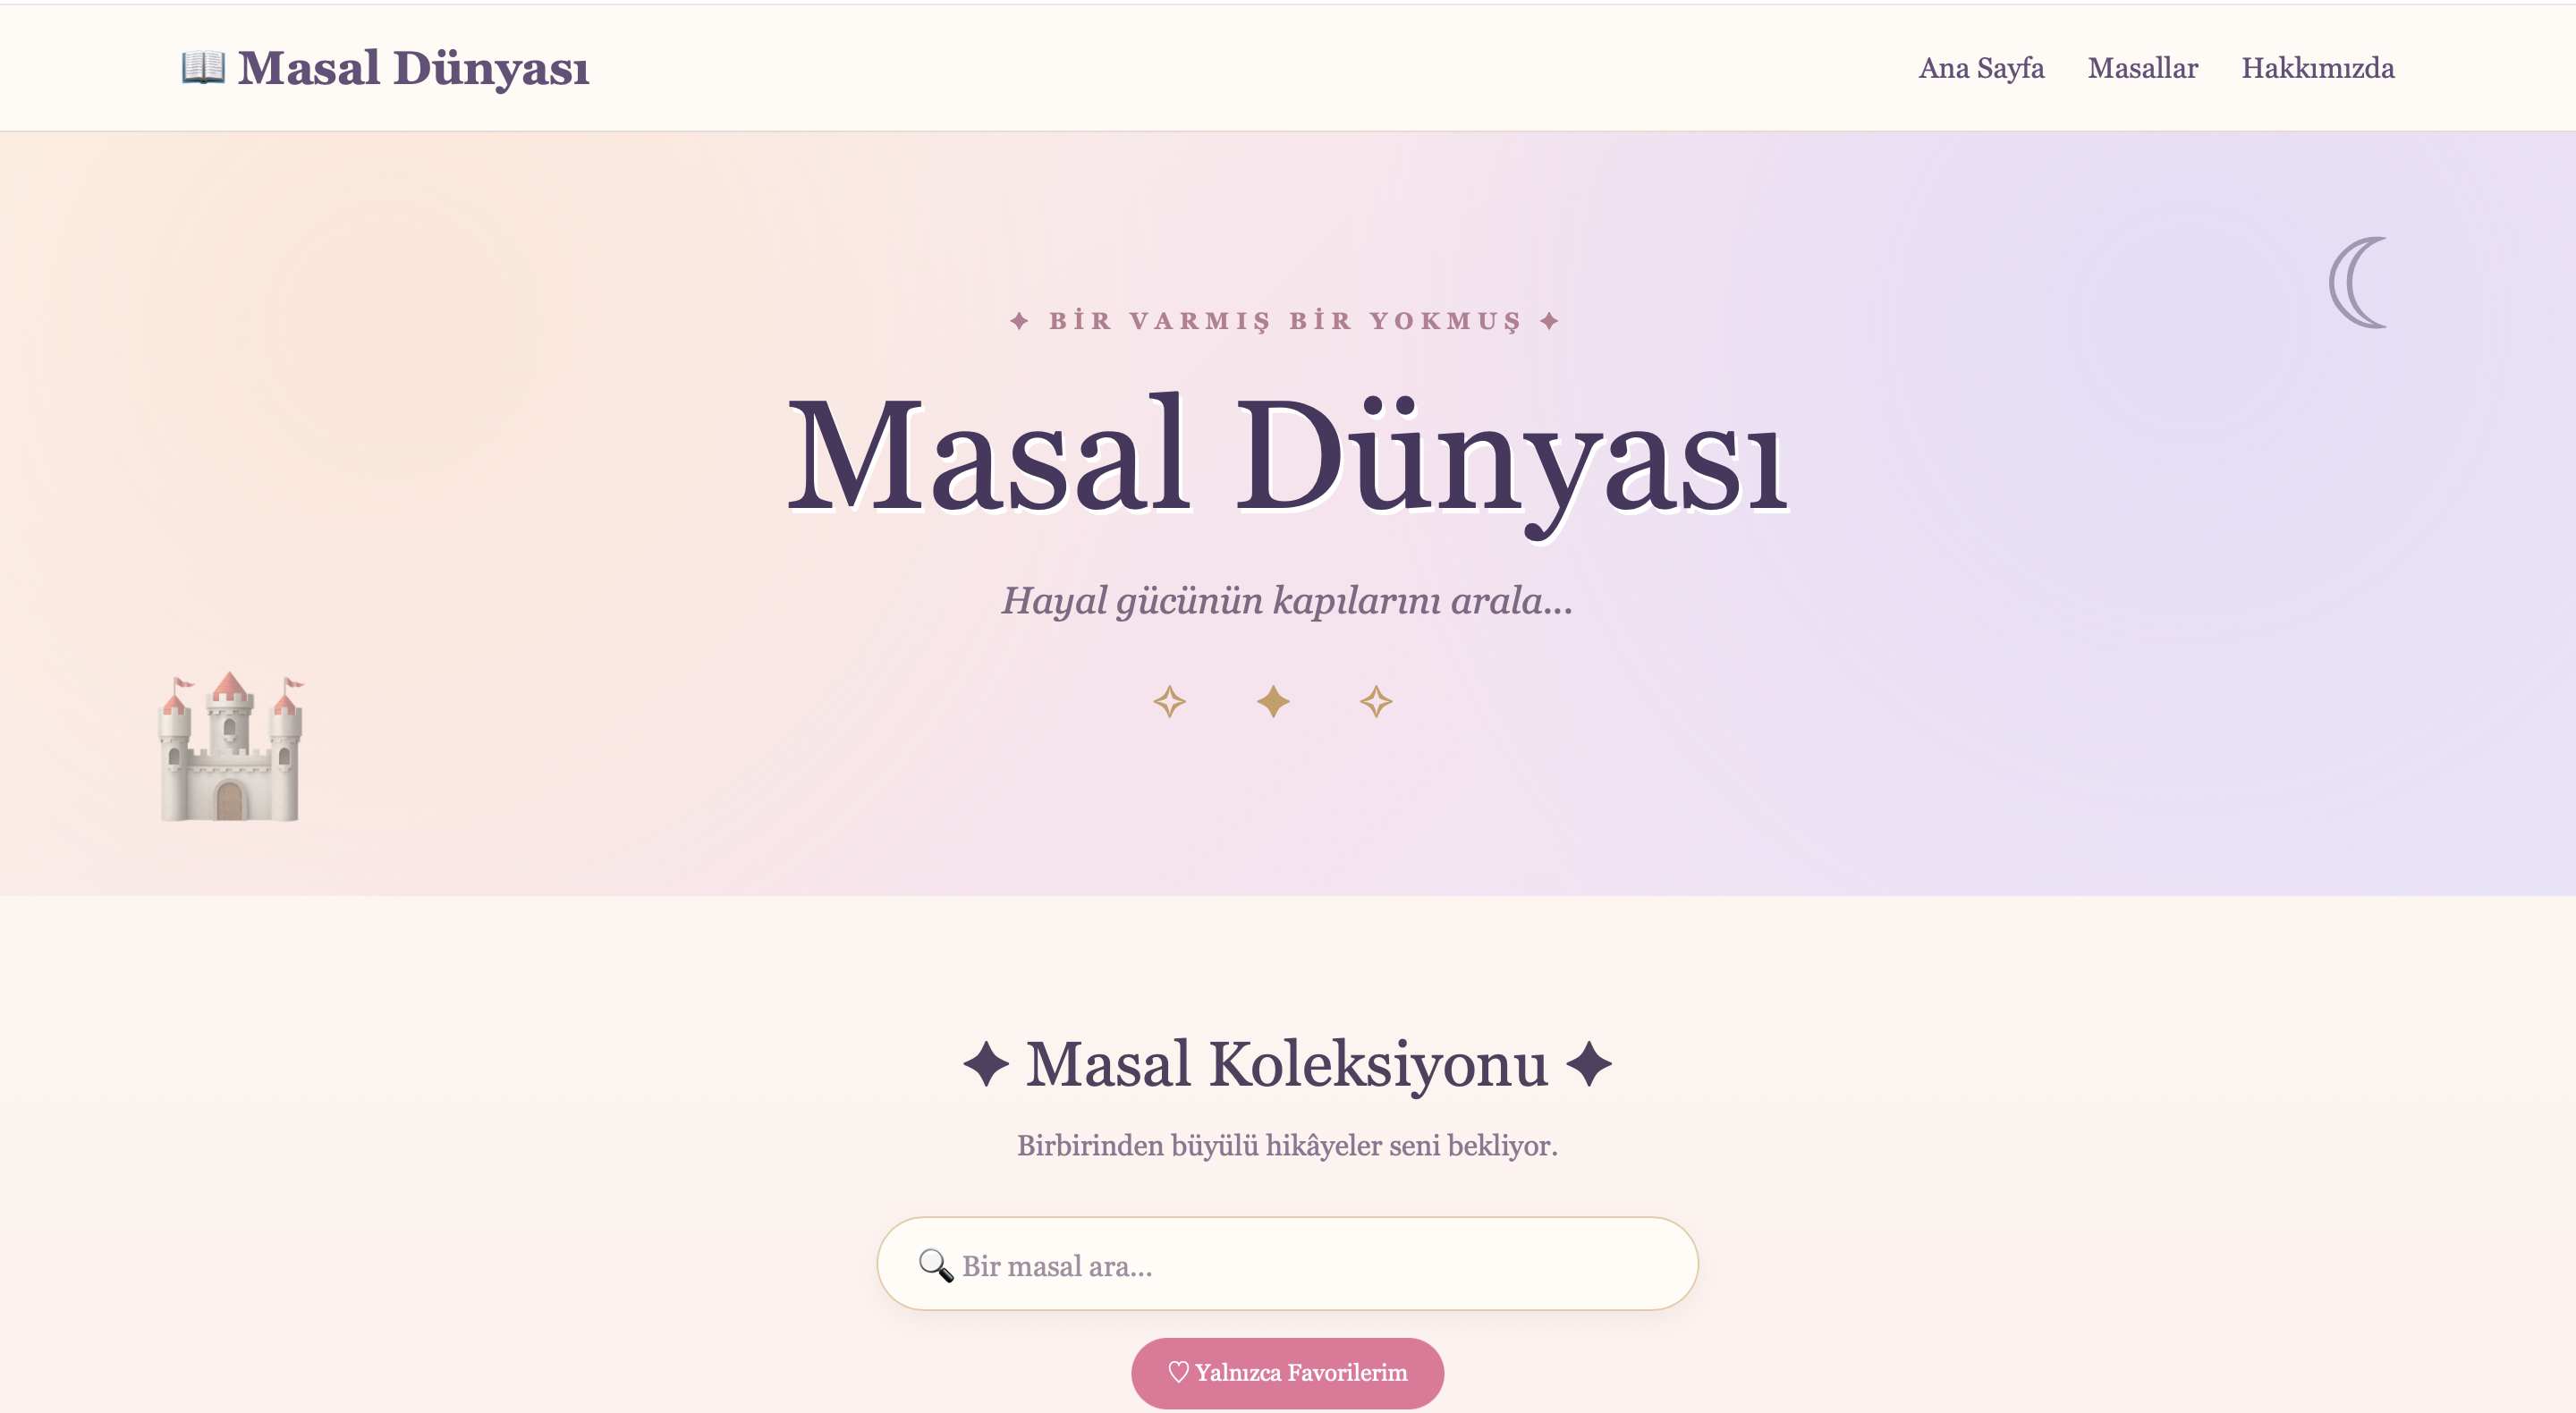
\includegraphics{anasayfa.png}
\caption{Ana sayfa görünümü}
\end{figure}

\begin{figure}[p]
\centering
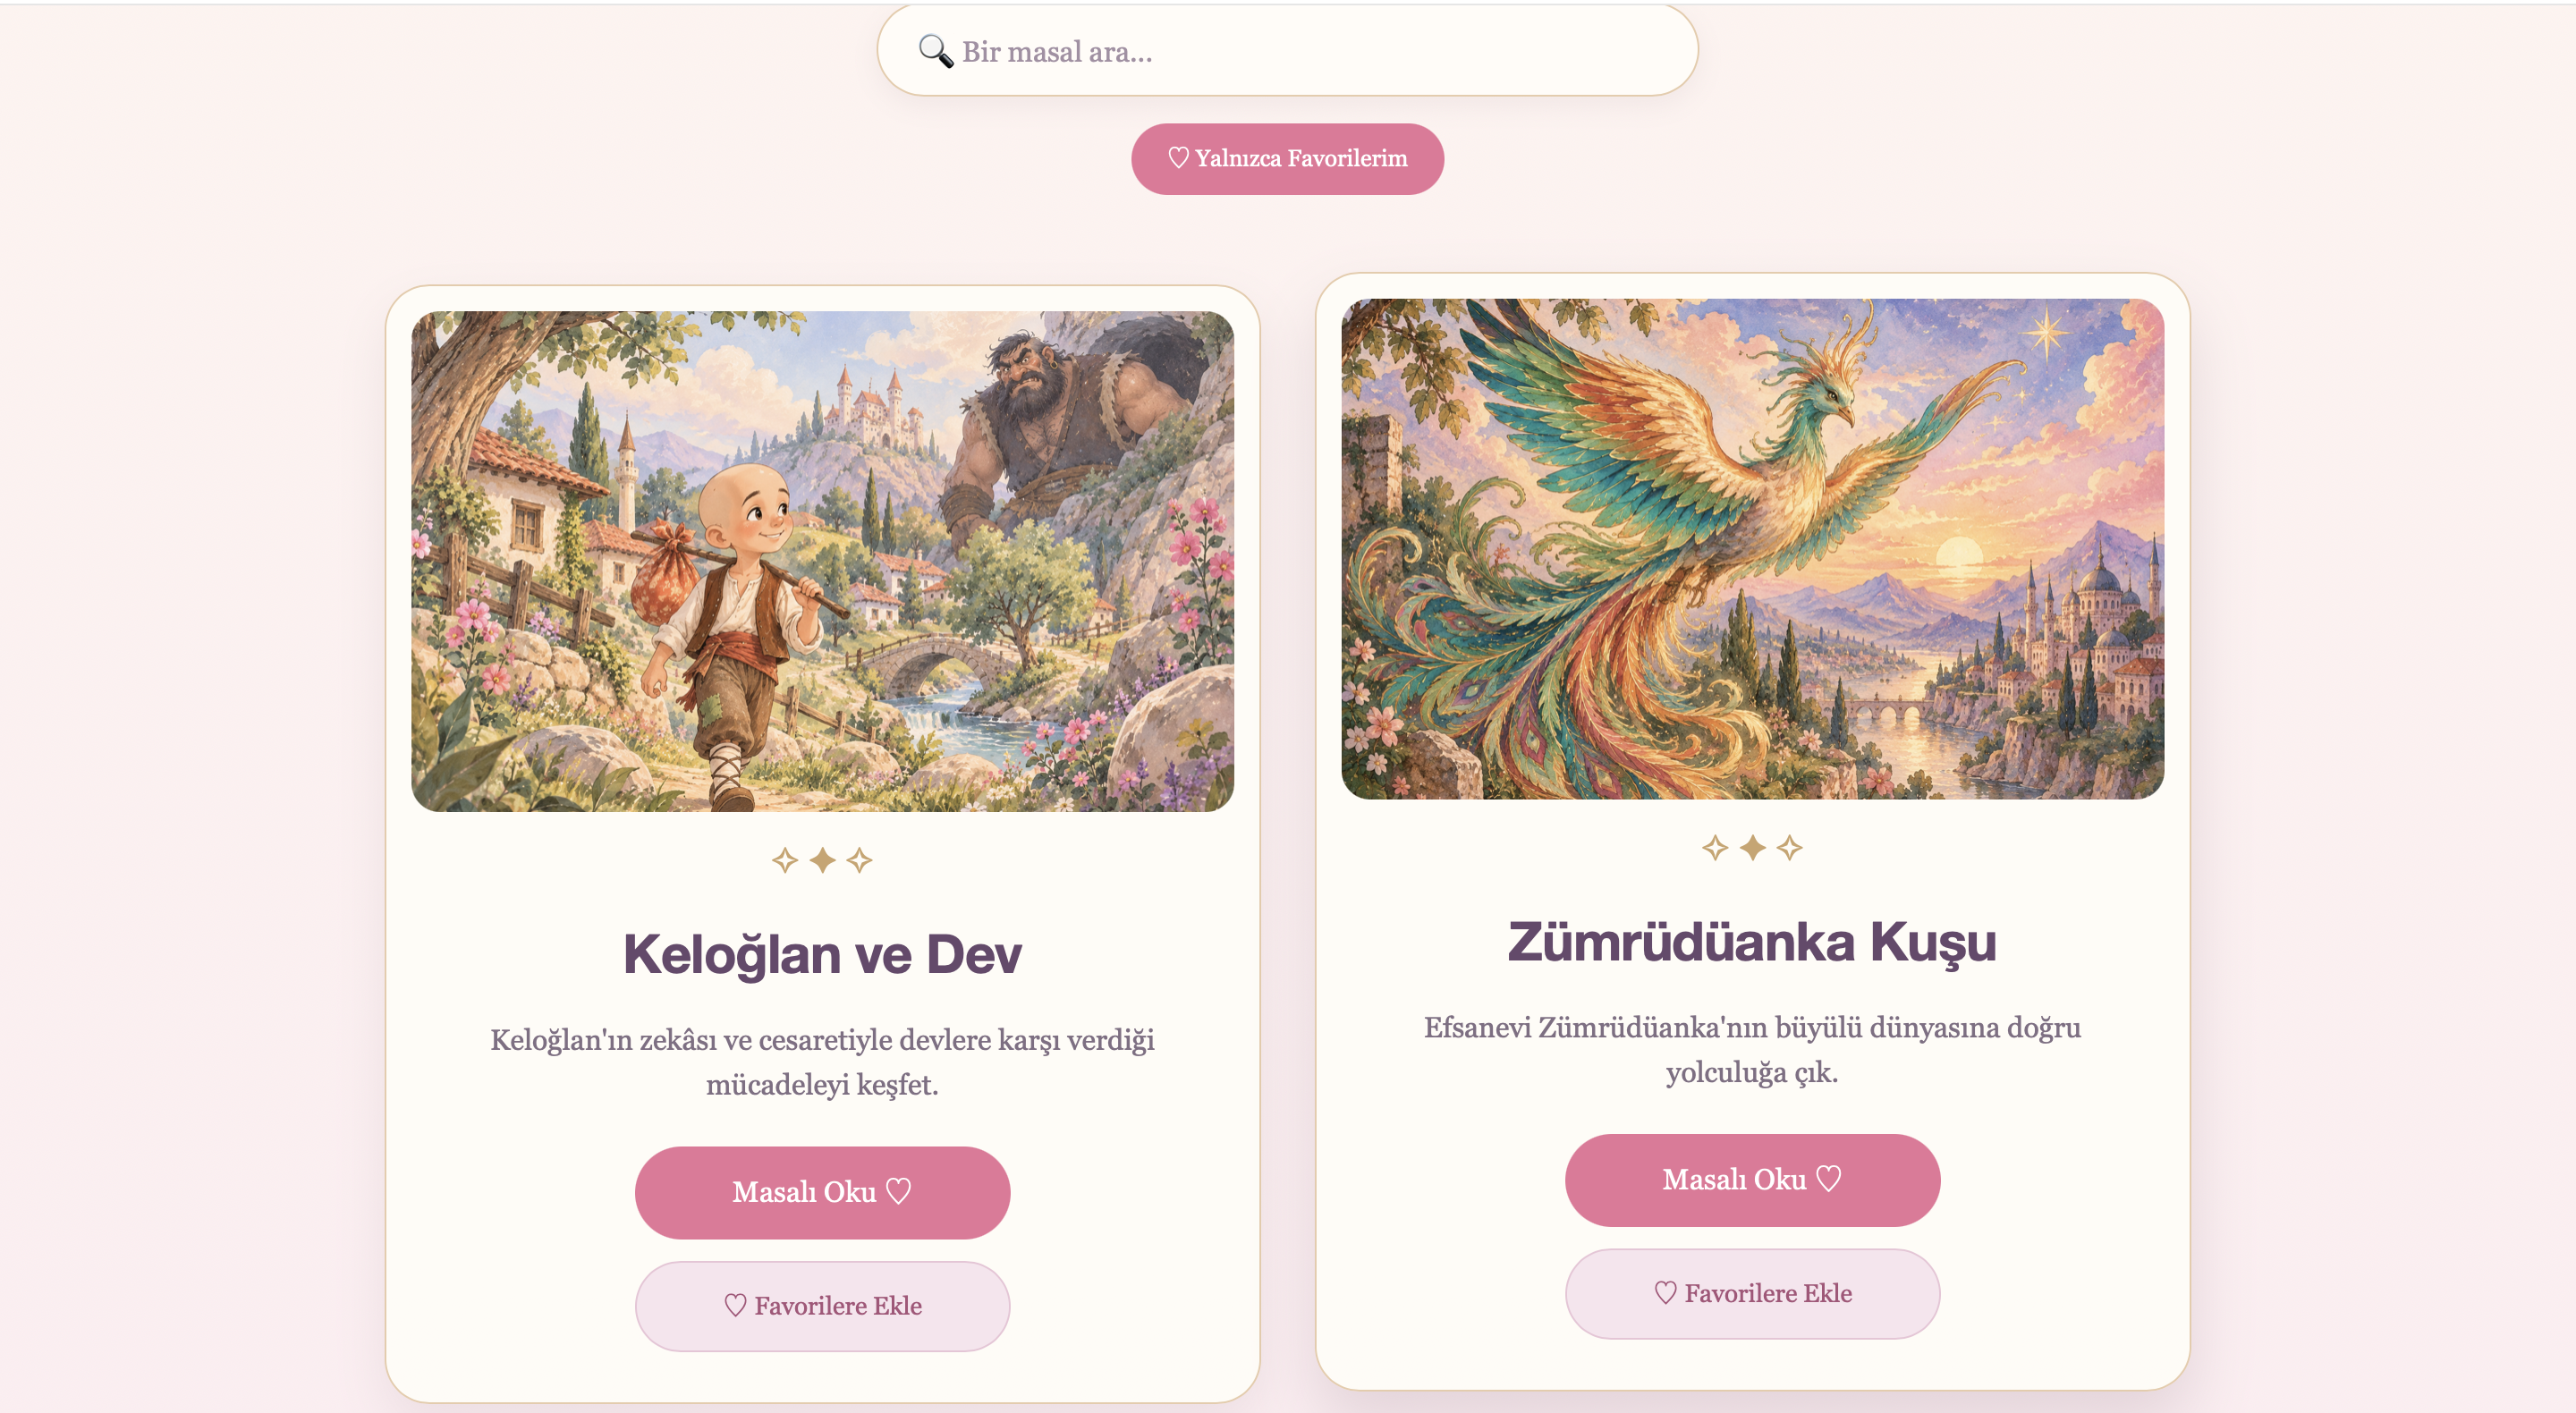
\includegraphics{masallar.png}\caption{Masal kartları}
\end{figure}

\begin{figure}[p]
\centering
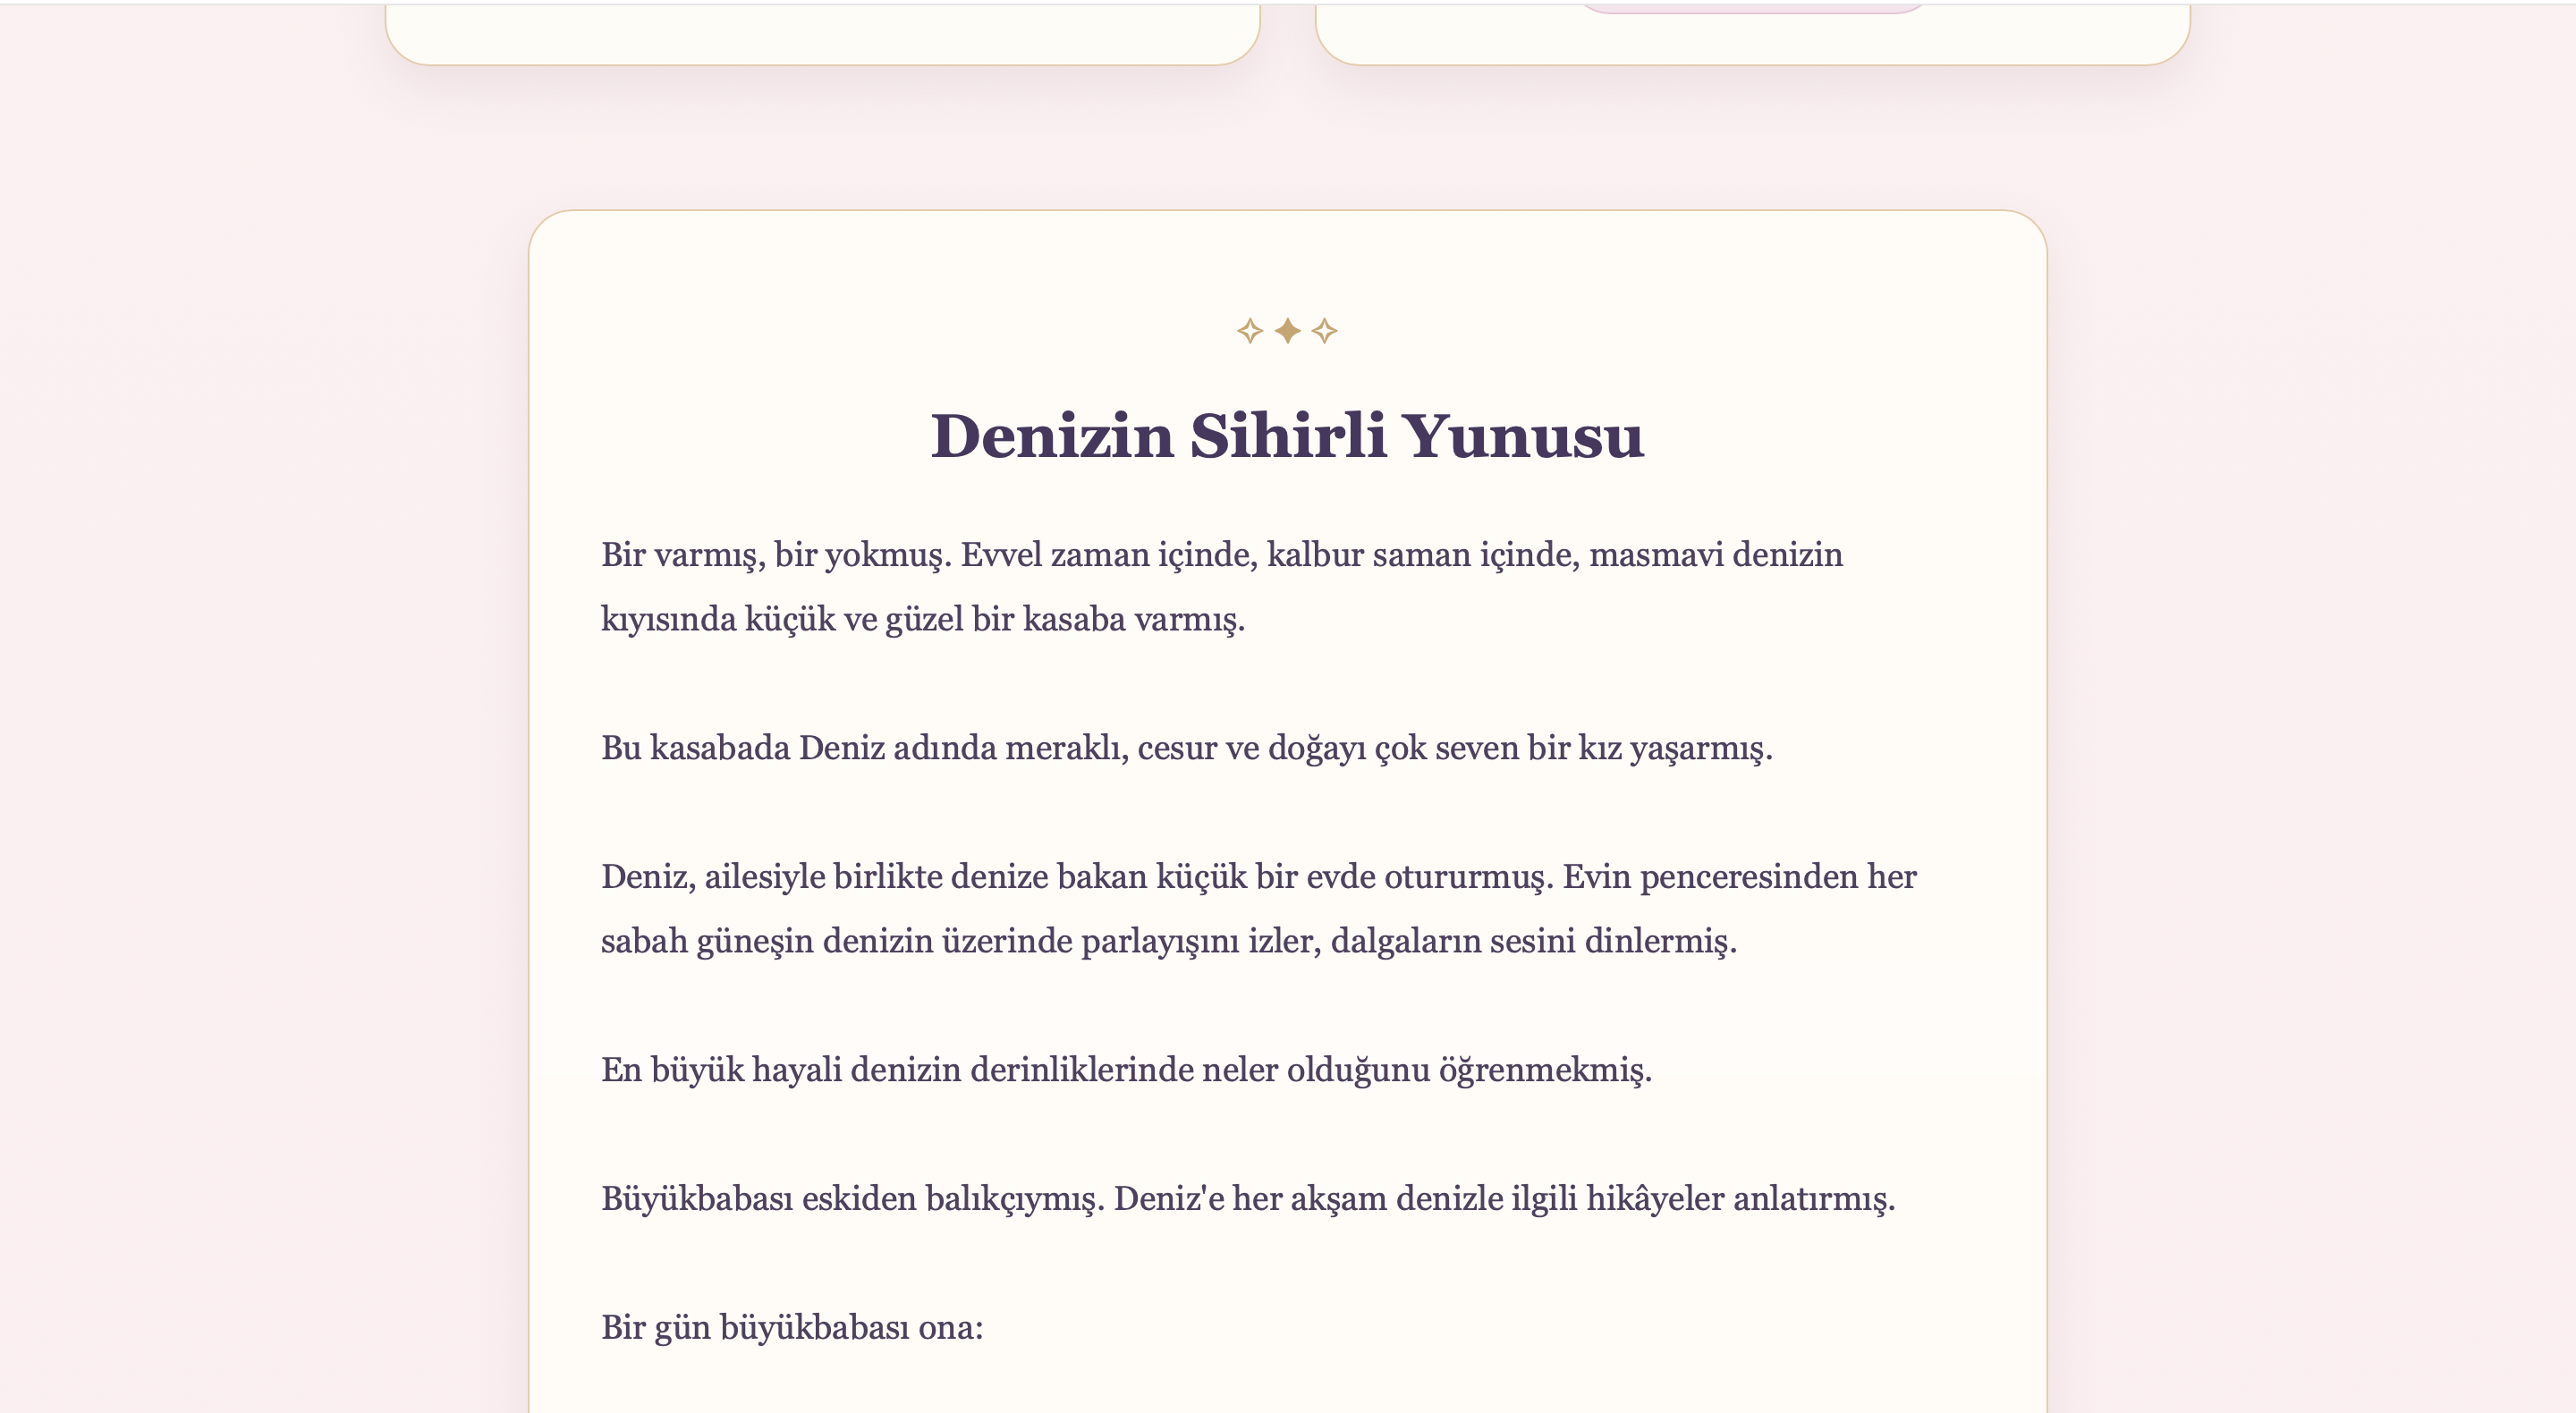
\includegraphics{okuma.png}
\caption{Masal okuma alanı}
\end{figure}

\begin{figure}[p]
\centering
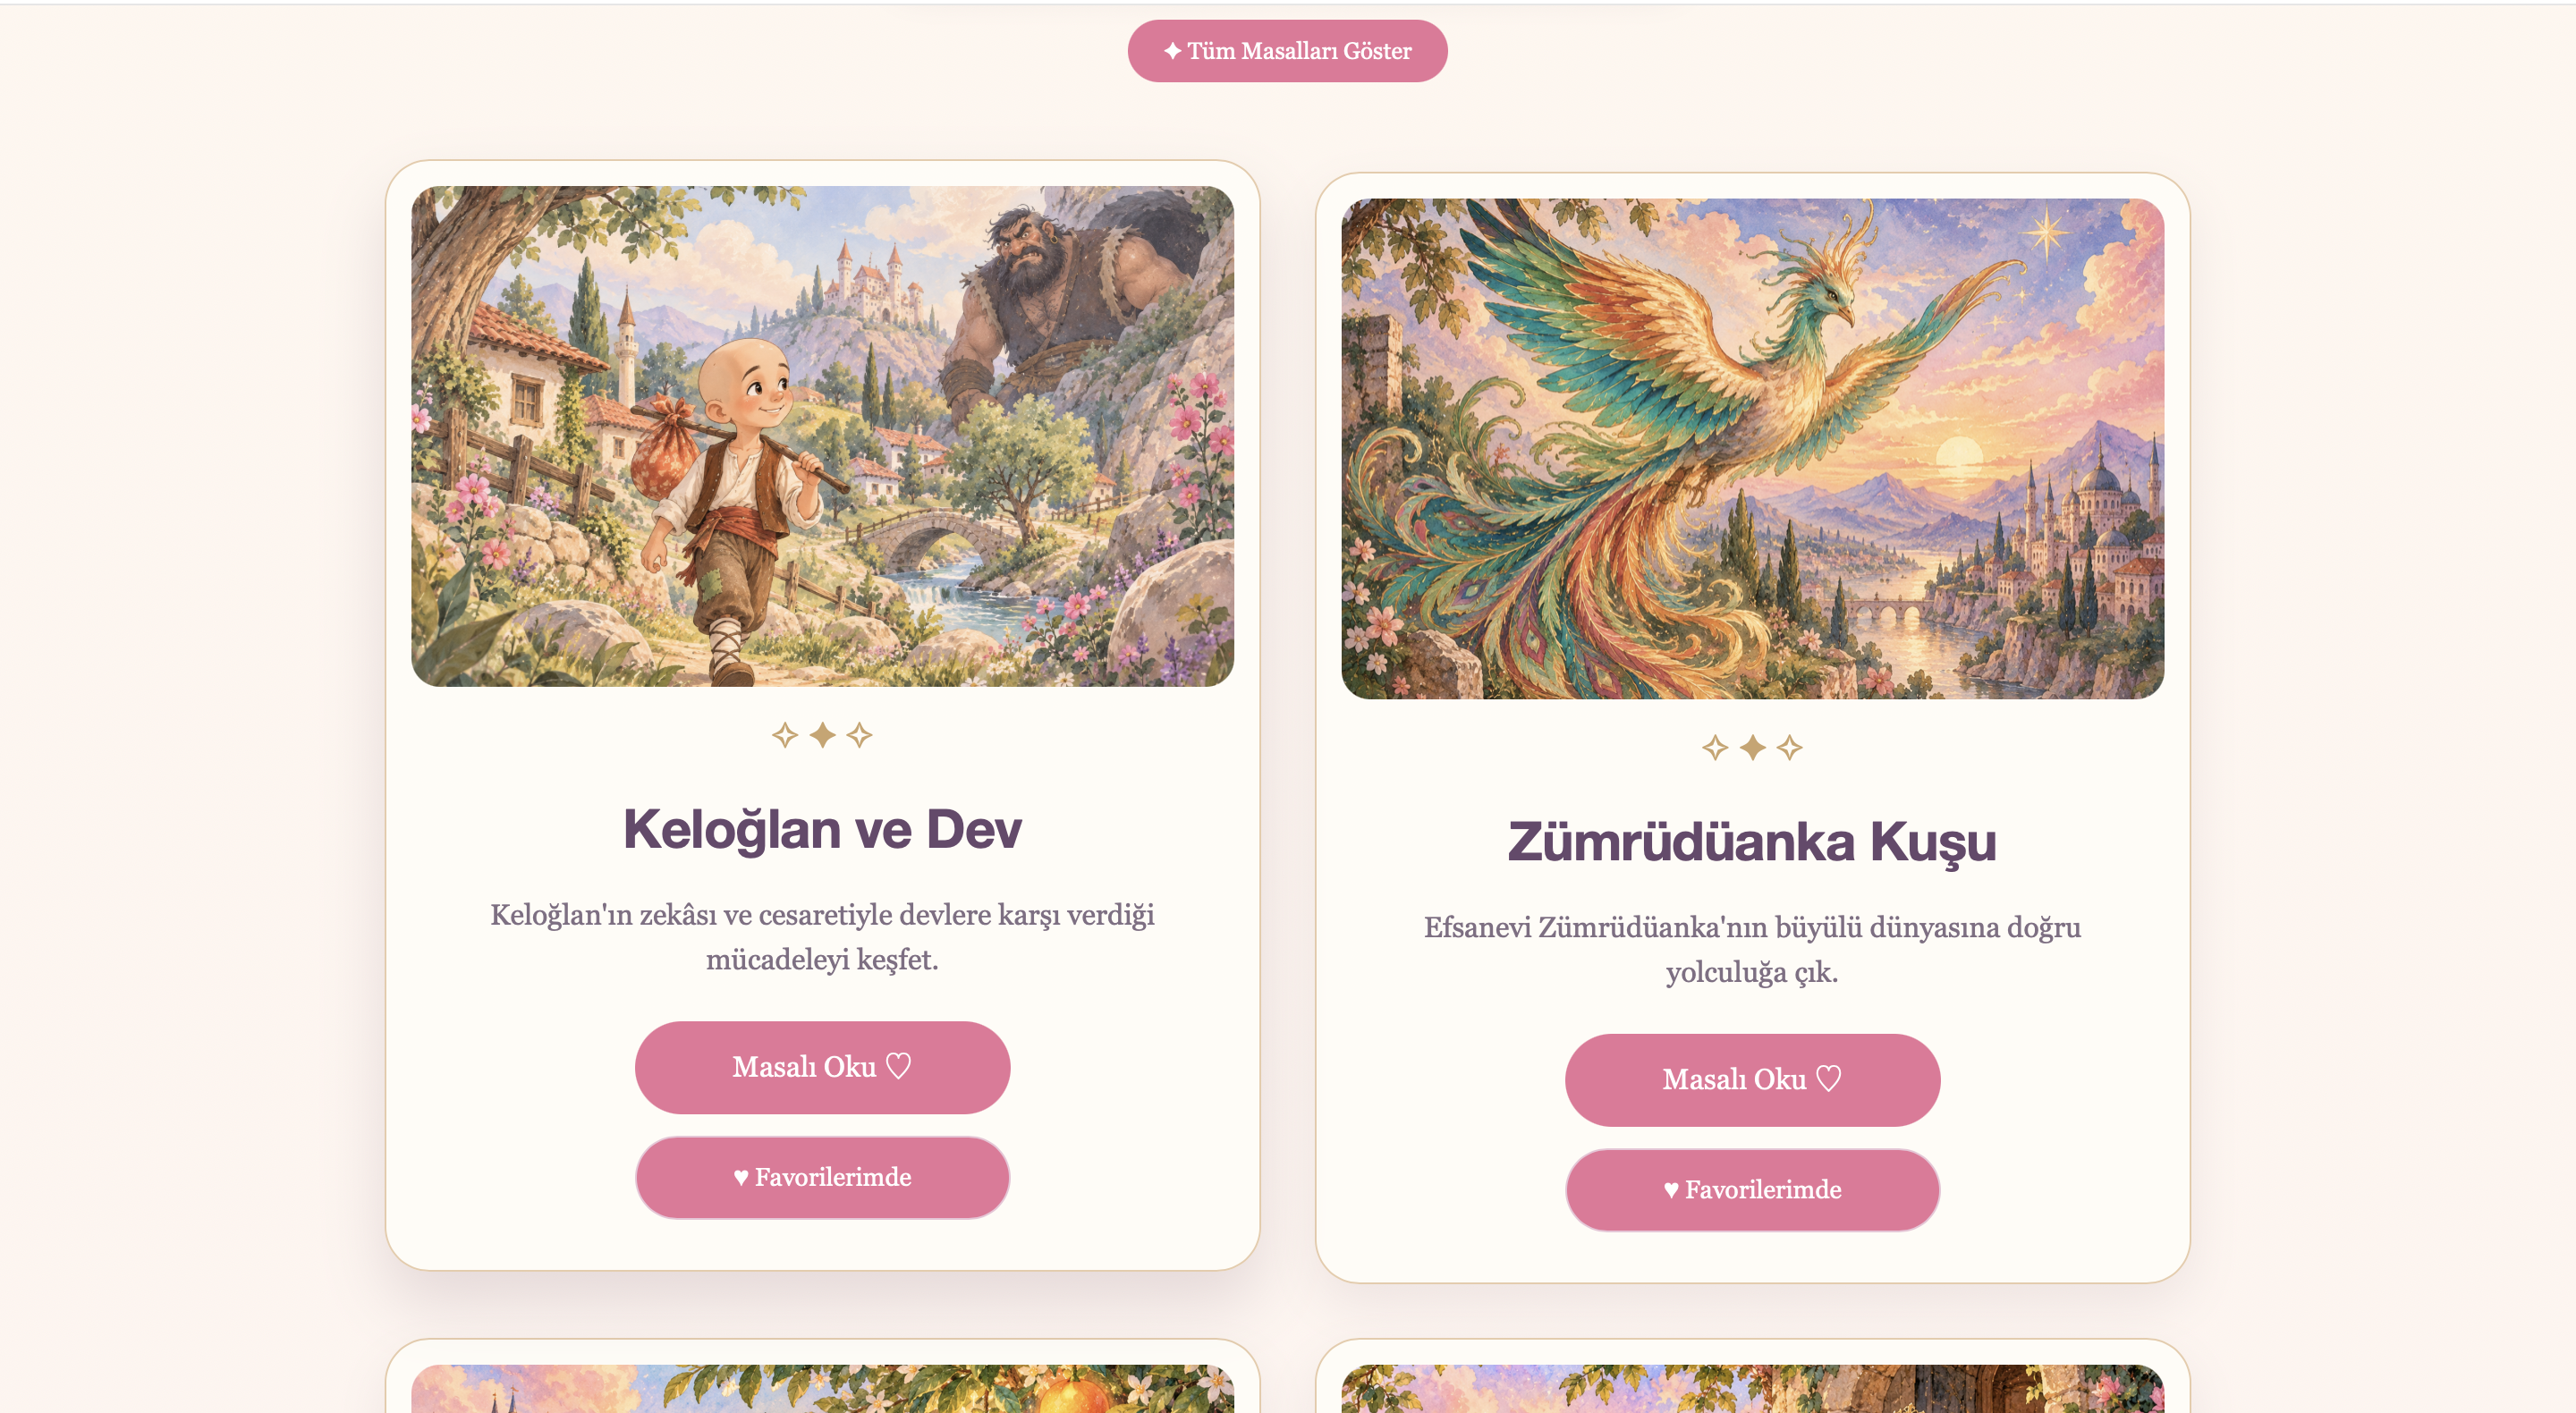
\includegraphics{favoriler.png}
\caption{Favori masallar}
\end{figure}

\begin{figure}[p]
\centering
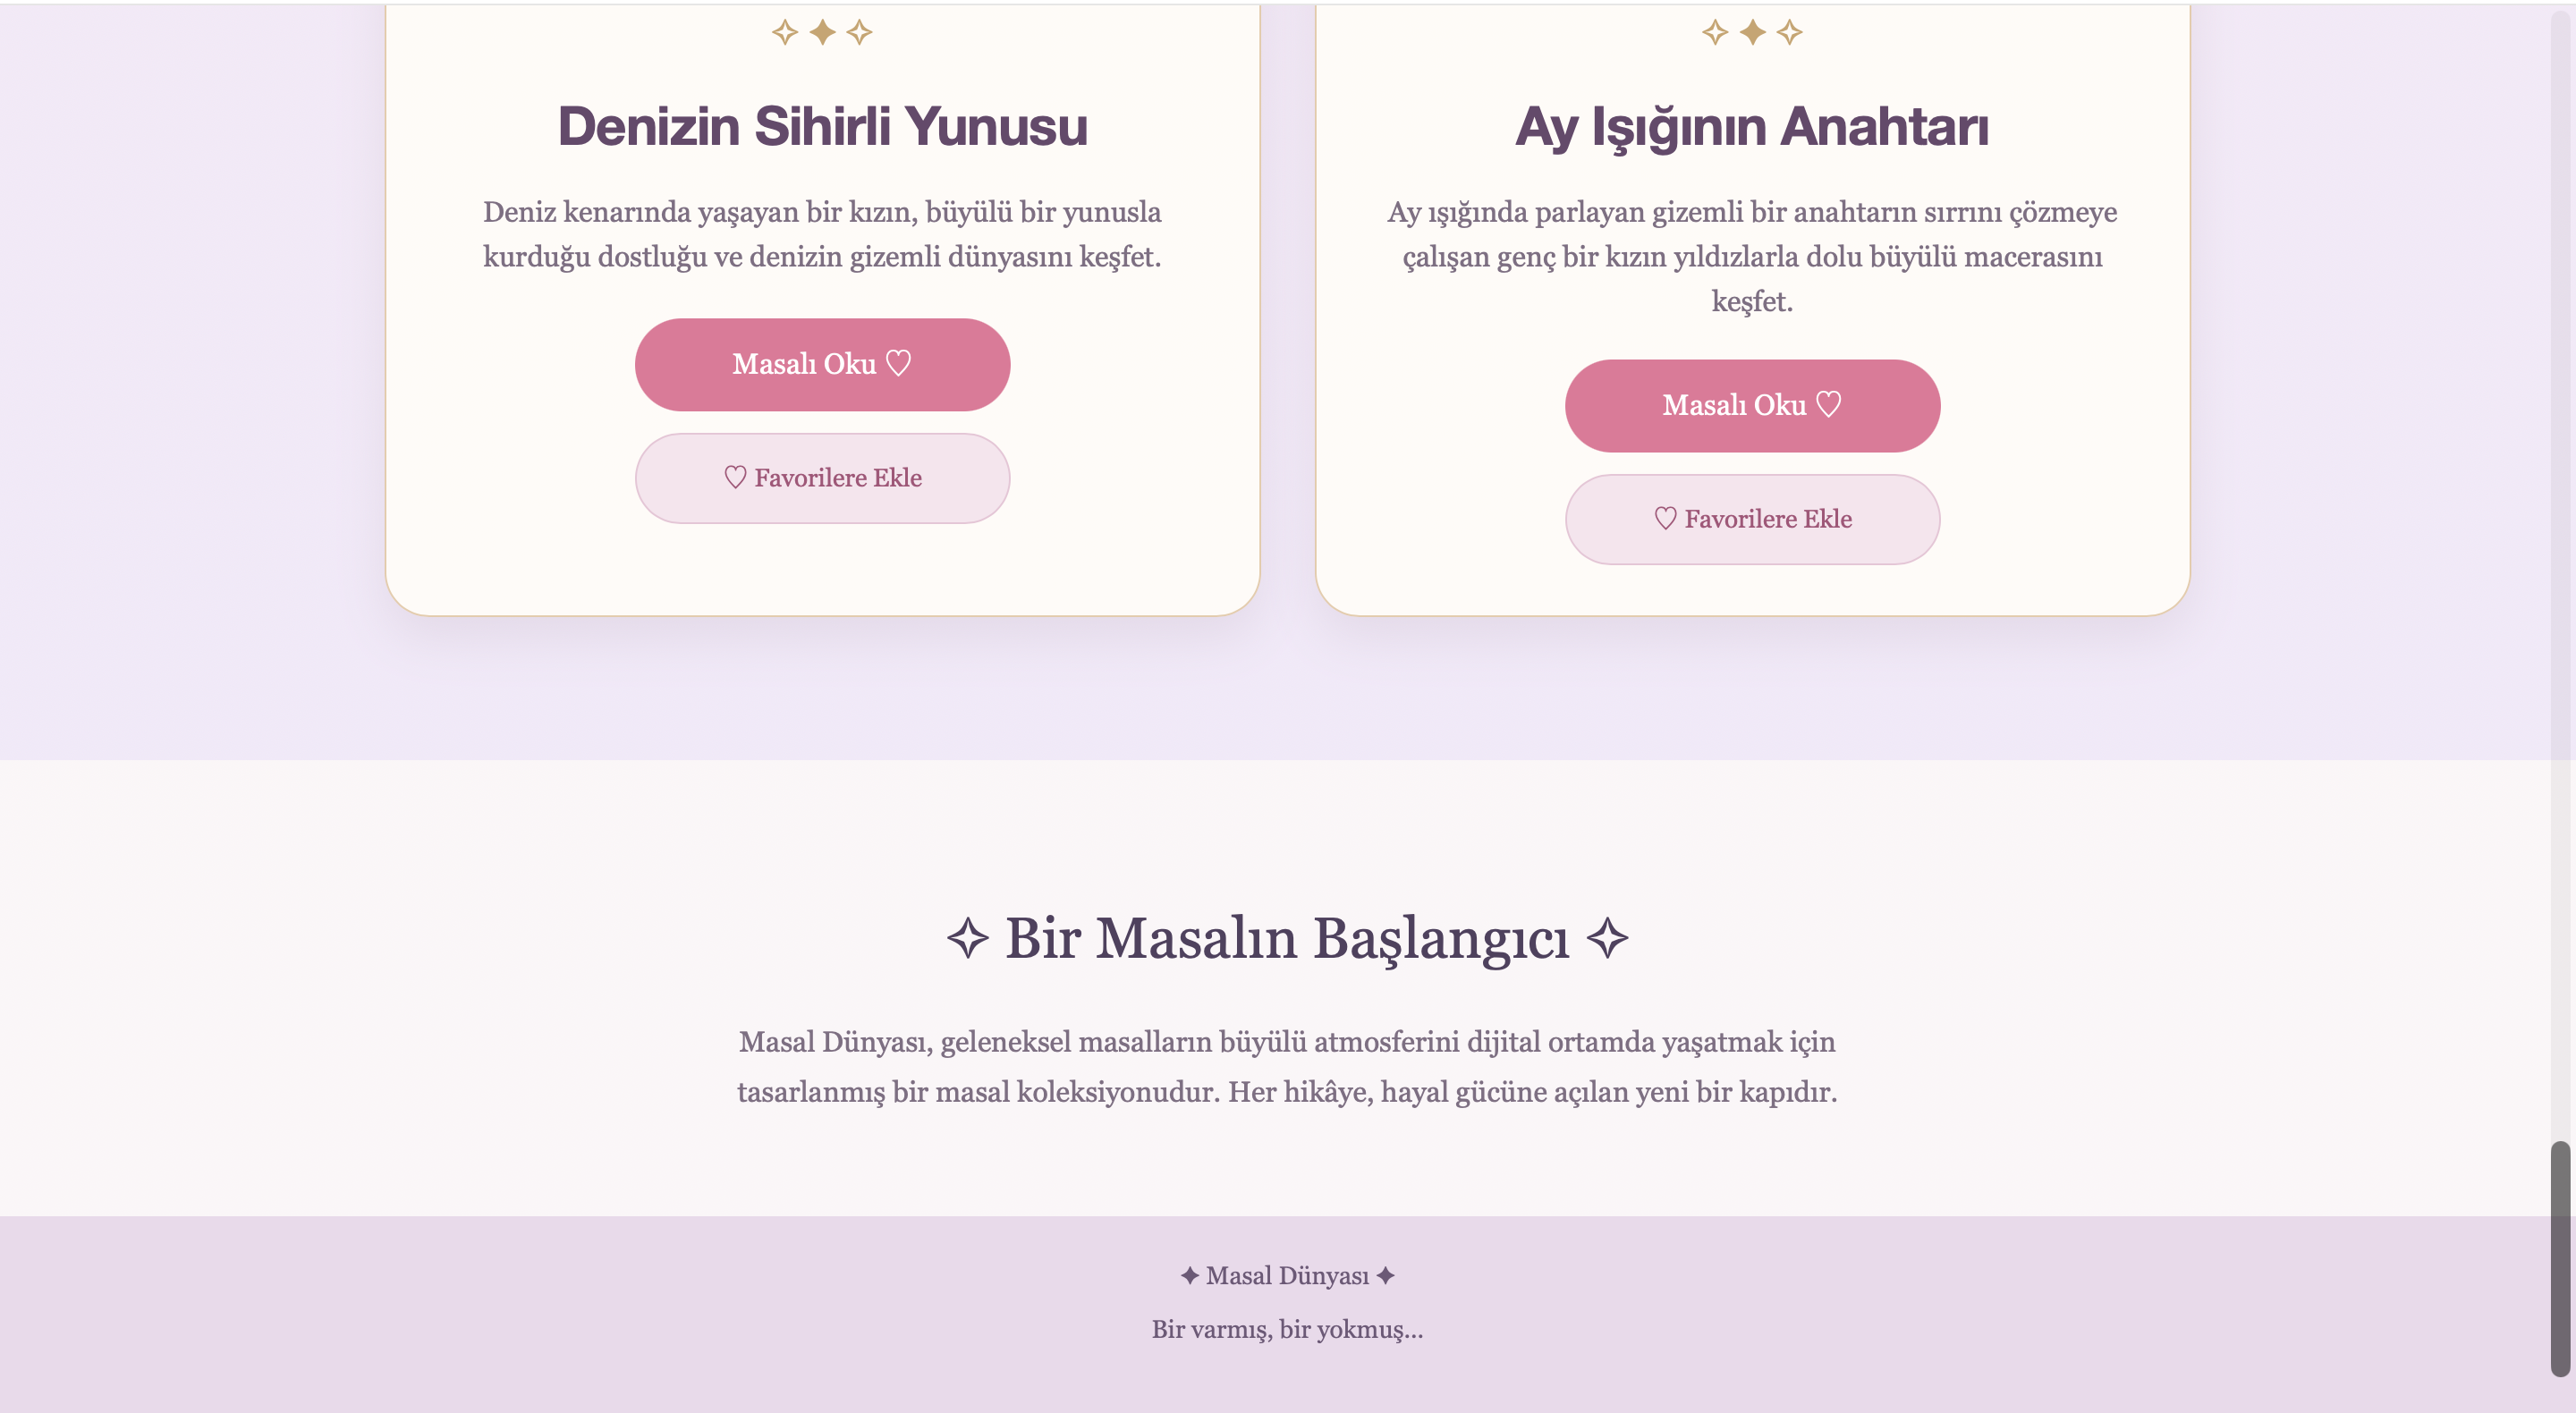
\includegraphics{sayfasonu.png}
\caption{Sayfanın alt bölümü}
\end{figure}
 \clearpage

\begin{figure}[p]
\centering
\resizebox{!}{0.70\textheight}{%
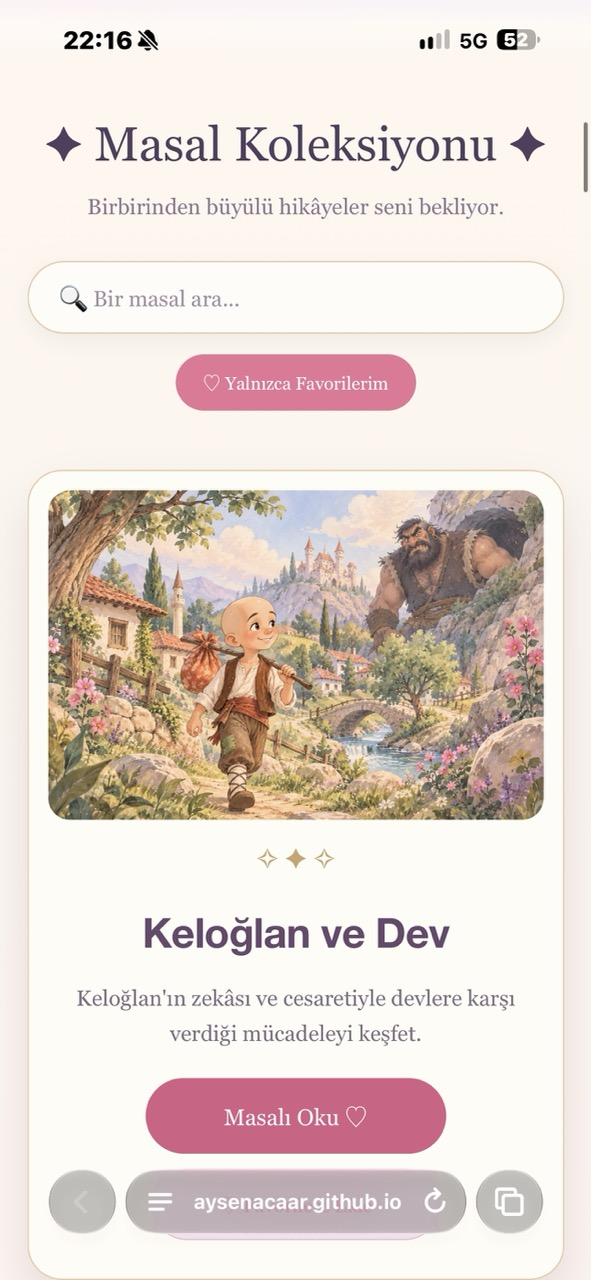
\includegraphics{mobilgorunum.jpg}%
}
\caption{Masal Dünyası web sitesinin mobil görünümü}
\label{fig:mobilgorunum}
\end{figure}
 \clearpage
 
%

\section{Gerçekleştirme}
% ====================================================================
\aciklama{Masal Dünyası web sitesini HTML, CSS ve JavaScript kullanarak oluşturdum. HTML ile sayfanın temel yapısını hazırladım. Sayfada üst menü, giriş alanı, masal kartları, masal okuma bölümü ve alt bilgi alanı bulunmaktadır. Toplam 10 masal için ayrı kartlar oluşturdum. Her kartta masalın görseli, adı, kısa açıklaması ve ilgili butonlar yer almaktadır.

CSS kullanarak web sitesinin renklerini, yazı tiplerini, kart tasarımlarını ve boşluklarını düzenledim. Masal atmosferine uygun olması için krem, pembe ve açık mor gibi pastel renkleri tercih ettim. Bilgisayarda masal kartları iki sütun hâlinde görünürken ekran küçüldüğünde tek sütuna geçecek şekilde duyarlı tasarım uyguladım.

JavaScript ile sayfanın etkileşimli özelliklerini hazırladım. Kullanıcı arama kutusuna bir masal adı yazdığında masalAra() fonksiyonu kartları kontrol ederek aramayla eşleşen masalları gösterir. Masal Oku butonuna basıldığında seçilen masalın metni okuma alanında açılır. Favorilere Ekle butonuyla beğenilen masallar favori olarak işaretlenebilir. Favorileri Göster özelliği ise yalnızca favori olarak seçilen masalları listeler. Böylece kullanıcılar istedikleri masallara daha kolay ulaşabilir.

Bu projede HTML sayfanın iskeletini, CSS görsel tasarımını, JavaScript ise kullanıcı etkileşimlerini sağlamaktadır. Kodları tek bir HTML dosyasında düzenleyerek sitenin internet bağlantısı gerektirmeden çalışmasını hedefledim.}

\subsection{HTML Yapısı}
Masal Dünyası web sitesinin temel yapısını HTML kullanarak oluşturdum. Sayfamı kullanıcıların kolayca gezinebileceği ve istedikleri masala rahatlıkla ulaşabileceği şekilde bölümlere ayırdım. Sayfanın üst kısmında `<nav>` etiketiyle oluşturduğum gezinme menüsü bulunmaktadır. Bu menüde Ana Sayfa, Masallar ve Hakkımızda bağlantıları yer almaktadır. `<header>` etiketiyle web sitesinin giriş bölümünü oluşturdum. Bu alanda sitenin başlığı ve masal dünyasını yansıtan tanıtım yazıları bulunmaktadır. Masalların bulunduğu ana içerik alanını `<main>` ve `<section>` etiketleriyle düzenledim. Her masalı ayrı bir `<article>` etiketi içerisinde hazırladım. Toplam 10 masal kartında masalın görseli, başlığı, kısa açıklaması, Masal Oku ve Favorilere Ekle butonları bulunmaktadır. Masal görsellerini `<img>`, başlıklarını `<h2>`, açıklamalarını `<p>` ve butonlarını `<button>` etiketleriyle ekledim. Kullanıcıların istedikleri masalı bulabilmesi için `<input>` etiketiyle bir arama kutusu oluşturdum. Seçilen masalın metninin görüntülendiği ayrı bir okuma alanı hazırladım. Sayfanın sonunda ise `<footer>` etiketiyle alt bilgi bölümünü oluşturdum. Bu HTML yapısı sayesinde web sitesinin bölümleri düzenli bir şekilde oluşturulmuş ve CSS ile JavaScript kodlarının bu bölümler üzerinde kullanılabilmesi sağlanmıştır.

\subsection{İçsel CSS}
Masal Dünyası web sitesinin görsel tasarımını HTML dosyasının içindeki `<style>` bölümünde CSS kullanarak oluşturdum. Masal atmosferine uygun krem, pastel pembe ve açık mor renklerini tercih ettim. Masal kartlarını CSS Grid ile bilgisayarda iki sütun hâlinde düzenledim. `@media` kuralını kullanarak ekran genişliği 700 pikselin altına düştüğünde kartların tek sütuna geçmesini sağladım. Böylece web sitesini farklı ekran boyutlarına uyumlu hâle getirdim.

\begin{lstlisting}[caption={İçsel CSS'ten önemli bir bölüm}]
.masallar {
    display: grid;
    grid-template-columns: repeat(2, minmax(0, 1fr));
    gap: 30px;
    max-width: 1050px;
    margin: 30px auto 60px;
    padding: 20px;
}

@media (max-width: 700px) {
    .masallar {
        grid-template-columns: 1fr;
        max-width: 500px;
    }
}
\end{lstlisting}

\subsection{Sayfanın Özellikleri}

Masal Dünyası web sitesini hazırlarken kullanıcıların masallara kolayca ulaşabileceği, hikâyeleri rahatlıkla okuyabileceği ve beğendikleri masalları seçebileceği etkileşimli bir yapı oluşturmaya çalıştım. Web sitesinde toplam 10 farklı masal bulunmaktadır. Her masal, kendisine ait illüstrasyon, başlık, kısa açıklama ve etkileşimli butonların bulunduğu bir kart içerisinde sunulmaktadır. Bu düzen sayesinde kullanıcılar masalları tek tek inceleyebilir ve ilgilerini çeken hikâyelere kolayca ulaşabilir.

Masal Arama Özelliği: Web sitesinin masal koleksiyonu bölümüne bir arama kutusu ekledim. Kullanıcılar bu alana okumak istedikleri masalın adını yazdıklarında JavaScript yardımıyla masal kartları filtrelenmektedir. Böylece kullanıcıların bütün masalları tek tek incelemesine gerek kalmadan aradıkları hikâyeye daha hızlı ulaşmalarını sağladım.

Masal Okuma Özelliği:Her masal kartında bulunan "Masalı Oku" butonuyla kullanıcılar seçtikleri hikâyenin tamamını okuyabilmektedir. Butona basıldığında ilgili masalın metni sayfa içerisinde bulunan okuma alanında görüntülenmektedir. Okuma işlemi tamamlandığında bu alan kapatılabilmektedir. Bu özellik sayesinde kullanıcılar farklı bir web sayfasına yönlendirilmeden masalları okuyabilmektedir.

Favorilere Ekleme Özelliği:Kullanıcıların beğendikleri masalları kolayca ayırt edebilmeleri için her masal kartına "Favorilere Ekle" butonu yerleştirdim. Bu butona basıldığında ilgili masal favori olarak işaretlenmektedir. Kullanıcı isterse aynı butonu kullanarak masalı favorilerinden çıkarabilmektedir. Böylece kullanıcıların kendi beğenilerine göre bir masal seçkisi oluşturması amaçlanmıştır.

Favorileri Filtreleme Özelliği:Masal koleksiyonu bölümünde bulunan "Yalnızca Favorilerim" butonuyla kullanıcılar yalnızca favori olarak işaretledikleri masalları görüntüleyebilmektedir. Bu özellik, özellikle daha önce beğenilen hikâyelere yeniden ulaşmayı kolaylaştırmaktadır.

Duyarlı Tasarım Özelliği: Web sitesini bilgisayar ve telefon ekranlarında kullanılabilecek şekilde tasarladım. CSS içerisinde kullandığım duyarlı tasarım kuralları sayesinde geniş ekranlarda masal kartları iki sütun hâlinde görüntülenirken küçük ekranlarda tek sütuna geçmektedir. Böylece sayfanın farklı cihazlarda düzenli ve okunabilir kalmasını hedefledim. Web sitesini bilgisayarda ve iPhone üzerinden Safari tarayıcısında test ederek masal kartlarının, görsellerin ve etkileşimli butonların çalıştığını kontrol ettim.

Görsel Tasarım ve Kullanıcı Deneyimi: Web sitesinin genelinde krem, pastel pembe ve açık lila renklerini tercih ettim. Masalların atmosferini desteklemek amacıyla her hikâye için özel illüstrasyonlar kullandım. Kartların benzer ölçülerde hazırlanmasına, yazıların okunabilir olmasına ve butonların kolay fark edilmesine dikkat ettim. Bu tasarım kararlarıyla hem masal dünyasına uygun bir görsel bütünlük oluşturmayı hem de kullanıcıların site içerisinde rahatça gezinmesini amaçladım.

Sonuç olarak HTML ile oluşturduğum sayfa yapısını CSS ile görsel açıdan düzenledim ve JavaScript kullanarak arama, favorilere ekleme, filtreleme ve masal okuma özelliklerini etkileşimli hâle getirdim. Böylece yalnızca masalları listeleyen bir sayfa yerine kullanıcıların seçim yapabildiği ve içeriklerle etkileşime girebildiği bir web sitesi hazırladım.

% ====================================================================
\section{Yapay Zekâ Kullanımı}
% ====================================================================
\aciklama {Web sitemde 10 farklı masal bulunmaktadır. Kullanıcılar masalları kartlar üzerinden inceleyebilir ve “Masalı Oku” butonuyla hikâyenin tamamını açabilir. Arama kutusuyla istedikleri masalı bulabilir, beğendikleri masalları favorilerine ekleyebilir ve yalnızca favorilerini görüntüleyebilirler. Ayrıca sayfa, farklı ekran boyutlarına uyum sağlayacak şekilde tasarlanmıştır.}

\begin{longtable}{@{}p{2.6cm}p{3.6cm}p{4.2cm}p{3.4cm}@{}}
\toprule

\textbf{Araç} & \textbf{Ne için kullandınız?} & \textbf{İstem (prompt) özeti} & \textbf{Sayfada nerede?} \\
\midrule
\endhead
\relax ChatGPT & Kod desteği ve metin düzenleme & Web sitesi için fikir alma, masallara uygun görseller oluşturma, yeni özellikler ekleme ve HTML, CSS ile JavaScript kodlarının nereye, nasıl yazılacağı konusunda yönlendirme alma. & HTML, CSS ve JavaScript \\

\relax ChatGPT & Masal görselleri & Masallara uygun, masalsı atmosferde illüstrasyonlar oluşturmak & Masal kartlarındaki görseller \\

\bottomrule
\end{longtable}

\subsection{Anladığım ve Kendim Yaptığım Kısımlar}
Projenin başlangıcında HTML, CSS ve JavaScript kodlarının nasıl kullanıldığını ve hangi kodun nereye yazılması gerektiğini öğrenmek için yapay zekâdan destek aldım. Özellikle ilk üç masalın kart yapısını oluştururken örneklerden yararlandım. Ancak bu süreçte kodları yalnızca kopyalamak yerine nasıl çalıştıklarını ve birbirleriyle nasıl bağlantı kurduklarını anlamaya çalıştım.

Dördüncü masaldan itibaren öğrendiğim yapıyı kendim uygulamaya başladım ve kalan masalları aynı sistem üzerinden bağımsız olarak ekleyebildim. Bu süreçte HTML etiketlerinin görevlerini, CSS ile görsel düzenin nasıl oluşturulduğunu ve JavaScript ile butonlara nasıl işlev kazandırıldığını daha iyi kavradım. Başlangıçta yapay zekâ desteğine ihtiyaç duyarken ilerleyen aşamalarda kendi başıma değişiklik yapabildiğimi görmek, programlama konusunda geliştiğimi fark etmemi sağladı. Bu proje sayesinde yalnızca bir web sitesi oluşturmayı değil, öğrendiğim kod yapısını anlayarak farklı içeriklere uygulamayı da öğrendim.

% ====================================================================
\section{Haftalık Katkılar}
% ====================================================================
\aciklama{Programlamaya Giriş dersini bir önceki dönemden tekrar almam ve eş zamanlı olarak özel sektörde bir şirkette görsel tasarımcı pozisyonunda aktif olarak çalışmam nedeniyle ders saatlerinde iş yerinde bulunmaktayım. Bu durum, derslere düzenli katılım sağlamamı güçleştirmektedir. Dersi tekrar alan bir öğrenci olarak devam zorunluluğumun bulunmadığı bilgisiyle hareket etmekle birlikte, dersin akademik gerekliliklerini ve öğrenme kazanımlarını yerine getirmeyi önemsiyorum.

Bu doğrultuda, ders kapsamında gerçekleştirilen uygulamaları ve verilen görevleri imkânlarım ölçüsünde takip ederek eksik çalışmalarımı bireysel olarak tamamlamaya, ders içi etkinlikleri sonradan telafi etmeye ve hazırladığım çalışmaları ilgili sisteme yüklemeye özen gösteriyorum.

Mesleki sorumluluklarım nedeniyle derslere eş zamanlı katılım sağlayamasam da öğrenme sürecinden kopmamaya, edindiğim bilgileri uygulamaya dönüştürmeye ve programlama alanındaki yetkinliklerimi geliştirmeye gayret gösteriyorum.

Bu açıklamayı, haftalık çalışmalarımın değerlendirilmesi sürecinde mevcut koşullarımın ve dersin gerekliliklerini yerine getirmek adına gösterdiğim bireysel çabanın da dikkate alınabilmesi amacıyla bilgilerinize sunmak isterim.}

\begin{longtable}{@{}>{\raggedright\arraybackslash}p{1.7cm}%
                    >{\raggedright\arraybackslash}p{6.4cm}%
                    >{\centering\arraybackslash}p{6cm}@{}}
\toprule
\rowcolor{ana}\textcolor{white}{\textbf{Hafta}} & \textcolor{white}{\textbf{Yapılan çalışma}} & \textcolor{white}{\textbf{Görsel}} \\
\midrule
\endfirsthead
\toprule
\rowcolor{ana}\textcolor{white}{\textbf{Hafta}} & \textcolor{white}{\textbf{Yapılan çalışma}} & \textcolor{white}{\textbf{Görsel}} \\
\midrule
\endhead
\bottomrule
\endfoot

\textbf{1. hafta}\newline 16 Eylül &
Bu hafta hazır HTML taslağında CSS kullanarak
arka plan rengini kırmızıya, yazı rengini
beyaza ve yazı tipini Helvetica olarak değiştirdim.
HTML yapısını koruyarak CSS ile görsel
düzenleme yapmayı öğrendim.
\newline
\textbf{Commit:} HTML taslağında renk ve font düzenlemeleri
\newline
$\square$ Ders içinde katılım sergiledim
\newline
$\boxtimes$ Telafi yaptım &
\haftagorsel{hafta1.png}\haftaek{hafta1b.png} \\
\midrule
\textbf{2. hafta}\newline 23 Eylül &
HTML ve CSS kullanarak moda temalı bir web sayfası hazırladım. Arka planı, yazı tiplerini ve renkleri düzenledim. Görsel ve bağlantılar ekledim.\newline
\textbf{Commit:} Moda temalı HTML ve CSS düzenlemeleri\newline
$\square$ Ders içinde katılım sergiledim\newline
$\boxtimes$ Telafi yaptım &
\haftagorsel{hafta2.png}\haftaek{hafta2b.png} \\
\midrule
\textbf{3. hafta}\newline 30 Eylül &
\textbf{1. Çalışma: HTML ve CSS}\newline
Hazır HTML sayfasında arka plan rengini, yazı tipini ve metin renklerini değiştirerek temel CSS özelliklerini uyguladım.\newline
\textbf{Commit:} HTML ve CSS stil düzenlemeleri\newline

\textbf{2. Çalışma: JavaScript}\newline
JavaScript ile bir sayacı 10 artıran, 10 azaltan ve sıfırlayan butonlar oluşturdum. Butonlara tıklandığında ekrandaki sayının nasıl değiştiğini öğrendim.\newline
\textbf{Commit:} JavaScript sayaç uygulaması\newline

$\square$ Ders içinde katılım sergiledim\newline
$\boxtimes$ Telafi yaptım
&
\begin{minipage}{\linewidth}
\centering
\haftagorsel{hafta3.png}

\vspace{0.4cm}

\haftagorsel{hafta3.2.png}
\end{minipage}
\\
\midrule
\textbf{4. hafta}\newline 7 Ekim &
\textbf{1. Çalışma: Buton ve Mesaj Gösterimi}\newline
JavaScript ile bir butona tıklandığında ekranda bilgilendirme mesajı gösteren bir uygulama hazırladım.\newline

\textbf{2. Çalışma: Kıyafet Sayacı}\newline
İhtiyaç sahipleri için kıyafet sayısını artırıp azaltan bir sayaç oluşturdum. CSS ile arka plan rengini düzenledim.\newline

\textbf{3. Çalışma: Kullanıcı Karşılama}\newline
Kullanıcının adını alarak kişiye özel karşılama mesajı gösteren ve boş girişleri kontrol eden bir uygulama geliştirdim.\newline

\textbf{Commit:} JavaScript buton, sayaç ve kullanıcı girişi çalışmaları\newline
$\square$ Ders içinde katılım sergiledim\newline
$\boxtimes$ Telafi yaptım
&
\begin{minipage}{\linewidth}
\centering
\haftagorsel{hafta4.png}

\vspace{0.3cm}

\haftagorsel{hafta4.2.png}

\vspace{0.3cm}

\haftagorsel{hafta4.3.png}
\end{minipage}
\\
\midrule
\textbf{5. hafta}\newline 14 Ekim &
\textbf{1. Çalışma: Sipariş Onay Butonu}\newline
JavaScript kullanarak butona tıklandığında ekranda sipariş bilgilendirme mesajı gösteren bir uygulama hazırladım.\newline

\textbf{2. Çalışma: Harry Potter Web Sayfası}\newline
HTML ve CSS kullanarak Harry Potter temalı bir web sayfası tasarladım. Arka plan, yazı tipleri, renkler, görsel ve metin düzenlemeleri yaparak sayfayı geliştirdim.\newline

\textbf{Commit:} Sipariş onay butonu ve Harry Potter temalı web sayfası\newline
$\square$ Ders içinde katılım sergiledim\newline
$\boxtimes$ Telafi yaptım
&
\begin{minipage}{\linewidth}
\centering
\haftagorsel{hafta5.png}

\vspace{0.3cm}

\haftagorsel{hafta5.2.png}
\end{minipage}
\\
\midrule
\textbf{6. hafta}\newline 21 Ekim &
\textbf{1. Çalışma: Moda Kategorileri}\newline
HTML ile elbise, çanta, ayakkabı, şal ve yeni sezon butonları oluşturdum. JavaScript'in onclick ve alert özelliklerini kullanarak butonlara tıklandığında ilgili mesajların görüntülenmesini sağladım.\newline

\textbf{2. Çalışma: Galatasaray Bağlantı Sayfası}\newline
HTML ile Galatasaray'ın resmî sitesine yönlendiren bir bağlantı ve marş arama butonu hazırladım. CSS ile arka plan ve yazı renklerini düzenledim. JavaScript kullanarak butona tıklandığında YouTube arama sayfasına yönlendirme ekledim.\newline

\textbf{Commit:} Moda kategorileri butonları ve Galatasaray bağlantı uygulaması\newline
$\square$ Ders içinde katılım sergiledim\newline
$\boxtimes$ Telafi yaptım
&
\begin{minipage}{\linewidth}
\centering
\haftagorsel{hafta6.png}

\vspace{0.3cm}

\haftagorsel{hafta6.2.png}
\end{minipage}
\\
\midrule
\textbf{7. hafta}\newline 28 Ekim &
\textbf{Moda Tasarımı Renk Uyumu Oyunu}\newline
HTML, CSS ve JavaScript kullanarak moda temalı bir renk uyumu oyunu hazırladım. Renk kutuları ve Minimal, Klasik, Sportif seçeneklerini oluşturdum. Kullanıcının seçimlerini değerlendiren ve puanını gösteren bir oyun yapısı geliştirdim.\newline

\textbf{Commit:} Moda temalı renk uyumu ve puanlama oyunu\newline
$\square$ Ders içinde katılım sergiledim\newline
$\boxtimes$ Telafi yaptım
&
\haftagorsel{hafta7.png}
\\
\bottomrule
\end{longtable}
% ==============================================================
\section{Test ve Değerlendirme}
% ====================================================================
\aciklama{Sayfayı hangi tarayıcı ve cihazlarda denediniz? Çalışmayan bir özellik
olduysa dürüstçe yazın ve nedenini açıklayın.}

\begin{center}
\rowcolors{2}{acik}{white}
\begin{tabular}{@{}p{6cm}p{3.4cm}p{3.4cm}@{}}
\toprule
\rowcolor{ana}\textcolor{white}{\textbf{Özellik}} & \textcolor{white}{\textbf{Bilgisayar}} & \textcolor{white}{\textbf{Telefon}} \\
\midrule
\relax Masal arama & Çalışıyor & Çalışıyor \\
\relax Favorilere ekleme & Çalışıyor  & Çalışıyor \\
\relax Masal okuma ve kapatma & Çalışıyor & Çalışıyor \\
\bottomrule
\end{tabular}
\end{center}

\textbf{Denenen tarayıcılar:} Chrome, Safari

% ====================================================================
\section{Sunum Videosu}
% ====================================================================
\begin{center}
\begin{tabular}{@{}ll@{}}
\textbf{Video süresi:} & [15 dakika 15 saniye] \quad \aciklama{12--18 dakika olmalıdır} \\
\textbf{Görünürlük:} & [Listelenmemiş / Herkese açık] \\
\textbf{Bağlantı:} & 

\ https://youtu.be/NXXDDQcXguQ \\
\end{tabular}
\end{center}

\subsection{Video Kontrol Listesi}
\aciklama{Teslimden önce hepsini kontrol edin ve kutuları $\boxtimes$ ile işaretleyin.}
\begin{itemize}
\item $\boxtimes$ Süre 12--18 dakika aralığında.
  \item $\boxtimes$ Sunum boyunca kameram açık, yüzüm görünüyor.
  \item $\boxtimes$ Görünürlük \textbf{Listelenmemiş} (ya da Herkese açık); \textbf{Özel} değil.
  \item $\boxtimes$ Bağlantıyı gizli pencerede açtım, video oynuyor.
  \item $\boxtimes$ YouTube videoyu işlemeyi bitirdi.
  \item $\boxtimes$ Videoyu baştan sona izledim; ses ve kamera tüm sunumda var.
  \item $\boxtimes$ Kapaktaki bağlantı ile bu bölümdeki bağlantı aynı.
\end{itemize}

% ====================================================================
\section{Sonuç ve Kendi Değerlendirmem}
% ====================================================================
\aciklama {Bu proje sayesinde HTML, CSS ve JavaScript'in bir web sayfası oluştururken nasıl birlikte çalıştığını daha iyi öğrendim. Başlangıçta kodların hangi bölümlere yazılması gerektiğini anlamakta ve sayfanın yapısını oluşturmakta zorlandım. Özellikle ilk üç masalı eklerken yapay zekâdan destek aldım ancak kodların çalışma mantığını öğrendikçe dördüncü masaldan itibaren diğer masalları kendi başıma ekleyebildim. CSS kullanarak renkleri, yazı tiplerini ve sayfa düzenini değiştirmeyi; JavaScript ile arama, favorilere ekleme ve masal okuma gibi etkileşimli özelliklerin nasıl çalıştığını öğrendim. En çok zorlandığım konulardan biri, yeni özellikler eklerken mevcut kod düzenini bozmadan doğru bölüme yerleştirmekti. Bu sorunu kodları inceleyerek, küçük değişiklikler yaparak ve sonuçlarını tarayıcıda kontrol ederek aşmaya çalıştım. Proje ilerledikçe başlangıçta karmaşık görünen kodları daha rahat okuyabildiğimi ve kendi başıma düzenlemeler yapabildiğimi fark ettim. İleride bu projeyi sesli masal anlatımı, yaş gruplarına göre filtreleme ve daha fazla masal seçeneği ekleyerek geliştirmek isterim. Bu çalışma, programlama konusunda kendime olan güvenimi artırırken öğrendiklerimi uygulamaya dönüştürmemi sağladı.}


% ====================================================================
\section{Kaynakça}
% ====================================================================
\aciklama{
\begin{itemize}
    \item \textbf{Masal Metinleri:} Türk masal anlatı geleneği ve masal türünün özellikleri temel alınarak metinler proje kapsamında yeniden düzenlenmiş ve özgün anlatımlarla hazırlanmıştır.

    \item \textbf{Masal Görselleri:} Projede kullanılan on masala ait illüstrasyonlar, yapay zekâ desteğiyle proje için özel olarak oluşturulmuştur. Görseller, masalların karakterlerine ve olay örgülerine uygun olacak şekilde hazırlanmıştır.

    \item \textbf{Yapay Zekâ Desteği:} OpenAI, ChatGPT. Proje kapsamında metin düzenleme, HTML, CSS ve JavaScript kodlarını anlama, geliştirme ve hata çözümleme aşamalarında destek amacıyla kullanılmıştır.

    \item \textbf{HTML Teknik Kaynağı:} MDN Web Docs, HTML. \url{https://developer.mozilla.org/en-US/docs/Web/HTML}

    \item \textbf{CSS Teknik Kaynağı:} MDN Web Docs, CSS. \url{https://developer.mozilla.org/en-US/docs/Web/CSS}

    \item \textbf{JavaScript Teknik Kaynağı:} MDN Web Docs, JavaScript. \url{https://developer.mozilla.org/en-US/docs/Web/JavaScript}
\end{itemize}
}
\begin{thebibliography}{9}

\bibitem{mdnhtml}
MDN Web Docs. HTML: HyperText Markup Language.
\url{https://developer.mozilla.org/en-US/docs/Web/HTML}

\bibitem{mdncss}
MDN Web Docs. CSS: Cascading Style Sheets.
\url{https://developer.mozilla.org/en-US/docs/Web/CSS}

\bibitem{mdnjs}
MDN Web Docs. JavaScript.
\url{https://developer.mozilla.org/en-US/docs/Web/JavaScript}

\bibitem{chatgpt}
OpenAI. ChatGPT.
Proje geliştirme sürecinde kodlama, metin düzenleme
ve hata giderme desteği.
\url{https://chatgpt.com/}

\bibitem{gorseller}
Proje Görselleri.
Masal Dünyası web sitesinde kullanılan 10 masal
illüstrasyonu, yapay zekâ desteğiyle proje
için özel olarak oluşturulmuştur.

\end{thebibliography}

% ====================================================================
\appendix
\section{Teslim Kontrol Listesi}
% ====================================================================
\aciklama{Teslim etmeden önce işaretleyin. Bu sayfayı teslim edilen PDF'te bırakabilirsiniz.}
\begin{itemize}  \item $\boxtimes$ MEBİS'e \textbf{yalnızca bu raporun PDF'ini} yükleyeceğim. ZIP ve HTML dosyası yüklemeyeceğim.
  \item $\boxtimes$ PDF dosya adı \texttt{OgrenciNo\_AdSoyad\_vize.pdf} biçiminde.
  \item $\boxtimes$ Kapaktaki GitHub ve YouTube bağlantıları doğru; PDF'te tıklayıp denedim.
  \item $\boxtimes$ GitHub deposunda web sayfası (tek \texttt{.html}), rapor PDF'i, \texttt{.tex} kaynakları ve \texttt{README.md} var.
  \item $\boxtimes$ GitHub deposu \textbf{herkese açık} (ya da öğretim üyesine erişim verdim).
  \item $\boxtimes$ Çalışmamın son hâli teslim saatinden \textbf{önce} depoya gönderildi (sonraki commitler değerlendirilmez).
  \item $\boxtimes$ Sayfa içsel CSS ve içsel JavaScript kullanıyor, harici dosya gerektirmiyor.
  \item $\boxtimes$ Hazır taslak kullanmadım; yapay zekâ kullandıysam Bölüm 5'i doldurdum.
  \item $\boxtimes$ Çalışmanın mantığını sunumda anlatabilirim.
\end{itemize}

\end{document}